%******************************************************************************%
%                                                                              %
%                  sample.en.tex for LaTeX                                     %
%                  Created on : Tue Mar 10 13:27:28 2015                       %
%                  Made by : David "Thor" GIRON <thor@42.fr>                   %
%                                                                              %
%******************************************************************************%

\documentclass{42-en}


%******************************************************************************%
%                                                                              %
%                                    Header                                    %
%                                                                              %
%******************************************************************************%
\begin{document}



                           \title{Structured Query Language: Intermediate!}
                          \subtitle{Beating a dead horse}
                       \member{Ted Tran}{ttran@student.42.us.org}
                        \member{42 figment of your imagination}{pedago@42.fr}

\summary {
  This project is the sequel to "Introduction to \texttt{SQL}".
}

\maketitle

\tableofcontents


%******************************************************************************%
%                                                                              %
%                                  Foreword                                    %
%                                                                              %
%******************************************************************************%
\chapter{Foreword}

\texttt{Zoomer}: \\
Refers to members of Generation Z and is a play on the term "Boomer," which refers to members of the Baby Boomer generation. The term Zoomer is also in reference to the fast-paced upbringings members of Generation Z are characterized to have due to the fast advances in technology and culture that has been happening around them as a result of the interconnectivity of the American and Global populations because of the ubiquity of internet-connected smart phones and social media.

Example of use in sentence: "I can't stand those Zoomers, all they do is use their phones all day to play Fortnite and watch TikTok videos!"

From \href{https://www.urbandictionary.com/define.php?term=Zoomer}{urbandictionary}.
    % Spacing in the source code does not influence spacing in the
    % generated pdf. The blank lines aboves and below won't appear.
    % Instead, use \newline (or its shortcut \\) and \newpage to
    % create vertical spacing.
    
            \begin{figure}[H]
                \begin{center}
                    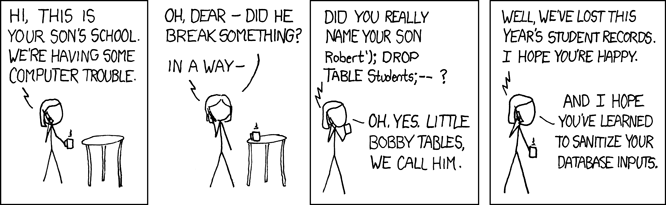
\includegraphics[width=17cm]{exploits.png}
                \end{center}
            \end{figure}

	    From xkcd! \\
	    	\newpage 	

%******************************************************************************%
%                                                                              %
%                                 Introduction                                 %
%                                                                              %
%******************************************************************************%
\chapter{Introduction}

	What the hell am I going to be doing?

	\begin{itemize}\itemsep1pt
		\item First, you're going to be running a ton of docker commands 
			so that you can run various things on these 42 lab computers
		\item Next, you're going to be building upon the SQL fundamentals you've learned. 
			You'll be reinforcing your fundamentals as well as building ontop of it. 
		\item Mhm, as usual it's time to write a ton of queries. Skill through experience!   
		\item Well, this time around, you'll be learning how to create your own database. 
			So, guess what the end goal is?
		\item You're going to create your own database! 
		\item After creating your database, you'll be filling it with data that you'll get 
			from web scraping, APIs, randomly generated, or just added manually.
		\item Then finally, it's time for you to create a wrapper so users can interact 
			with your database without writing SQL queries themselves. 
	\end{itemize}


	Testing is provided for you, so you only need to run a single command to 
	check your answers! Go for the green, buddy. 

%******************************************************************************%
%                                                                              %
%                                  Goals                                       %
%                                                                              %
%******************************************************************************%
\chapter{Goals}

	\begin{itemize}\itemsep1pt 
		\item Reinforce SQL fundamentals
		\item Learn MORE SQL, because this is a SQL project after all
		\item Learn how to create a database in Postgresql or Sqlite3
		\item Then use what you've learned at H2S to fill the database with... data!  
		\item Create a wrapper using a programming language of your choice, so 
			that a person can obtain information from your database without 
			having to write SQL queries themselves.
	\end{itemize}

	Your goal is to pass every single test for a beautiful 100 percent GREEN. Then 
	after that, use what you've learned at H2S to create your own database, seed it 
	with data, and create methods so users can interact with your DB without writing SQL queries! 

%******************************************************************************%
%                                                                              %
%                             General instructions                             %
%                                                                              %
%******************************************************************************%
\chapter{General instructions}

	\begin{itemize}\itemsep1pt 
		\item This project will be corrected by humans only. 
			You're allowed to organize and name your files as you see 
			fit, but you must follow the following rules. 
		\item The first rule of SQL Club is: You do not talk about SQL Club.
		\item The second rule of SQL Club is: You do not ta... wait, we did this already last time. 
			Well, this project's subtitle is beating a dead horse after all. 
		\item Within the mandatory part, you are only allowed to use SQL. 
		\item You can ask your questions on slack and random people in your nearby vicinity 
			that appear to be older than you. Of course, with the exception being me-- don't ask me 
			any questions. Everybody at 42 is a SQL master, and H2S mentors are required 
			to have a PhD in Structured Query Language studies! So don't be afraid to 
			come to them for guidance.
		\item The people who refused to give you help in the previous course were merely lazy. They dared to lie to your 
			face and say, "I don't know SQL!" so they could avoid helping you. Come after them with renewed vigor! 
		\item You will be provided with instructions on how to setup your programming environment, create the DB 
			and import data, a skeleton to code in, and a full testing suite to check your answers.
	\end{itemize}

% Don't forget this line for piscine days to initate the exercise counter at 0
\startexercices

%******************************************************************************%
%                                                                              %
%                             THE SQL PISCINE LOL                              %
%                                                                              %
%******************************************************************************%

\chapter{Day \exercicenumber: Beginning your SQL studies! }

\extitle{SQL SELECT/FROM/WHERE, operators, DISTINCT, expression aliases, *}
\exfiles{01\_select.rb, 02\_select.rb, 03\_select.rb, 03a\_select.rb}
\exnotes{Make sure to use docker cp to store your files on the host computer, then add it to a git repo after!}
\makeheaderfiles

	Look at this example! \\
    
            \begin{figure}[H]
                \begin{center}
                    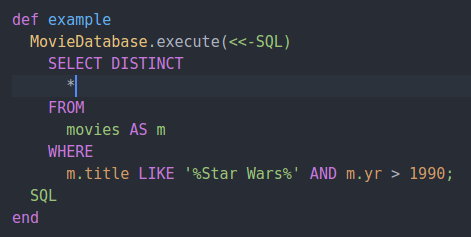
\includegraphics[width=14cm]{Ex00.png}
                \end{center}
            \end{figure}

	\begin{itemize}\itemsep1pt 
		\item SELECT chooses which columns to grab 
		\item FROM chooses which table to start from
		\item DISTINCT means you want this to be unique! No duplicates 
		\item * basically means that  you'll grab ALL. 
		\item You can aliases expressions or tables using "AS", this keeps your SQL code DRY. 
		\item WHERE is used to filter records by condition! 
		\item Now, what are some useful operators you can use in the WHERE clause?  
	\end{itemize}

    
            \begin{figure}[H]
                \begin{center}
                    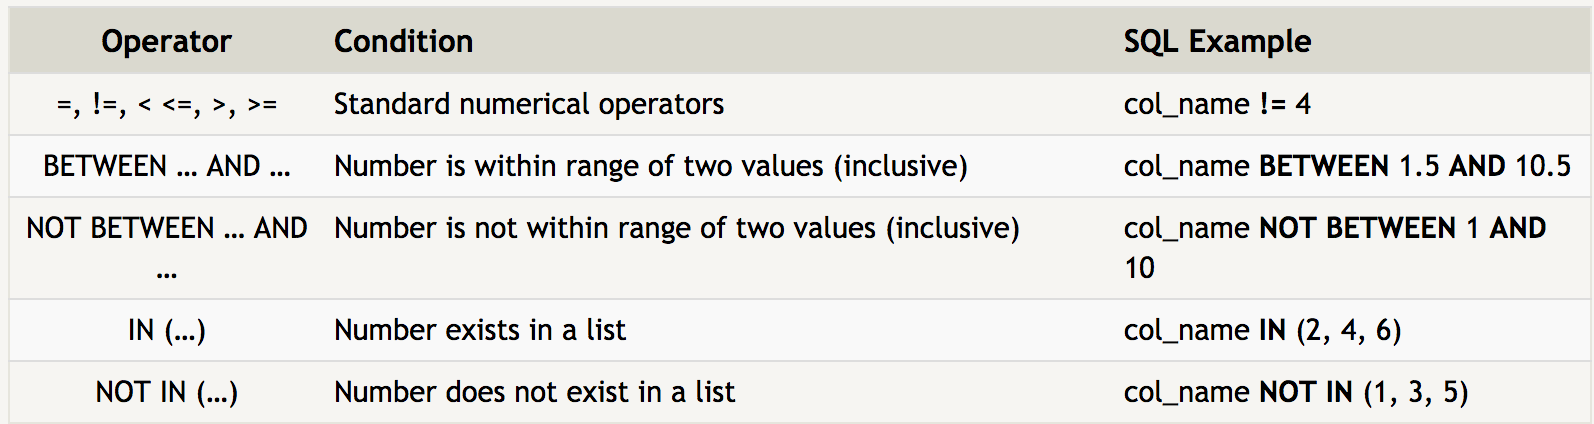
\includegraphics[width=14cm]{operators.png}
                \end{center}
            \end{figure}

    
            \begin{figure}[H]
                \begin{center}
                    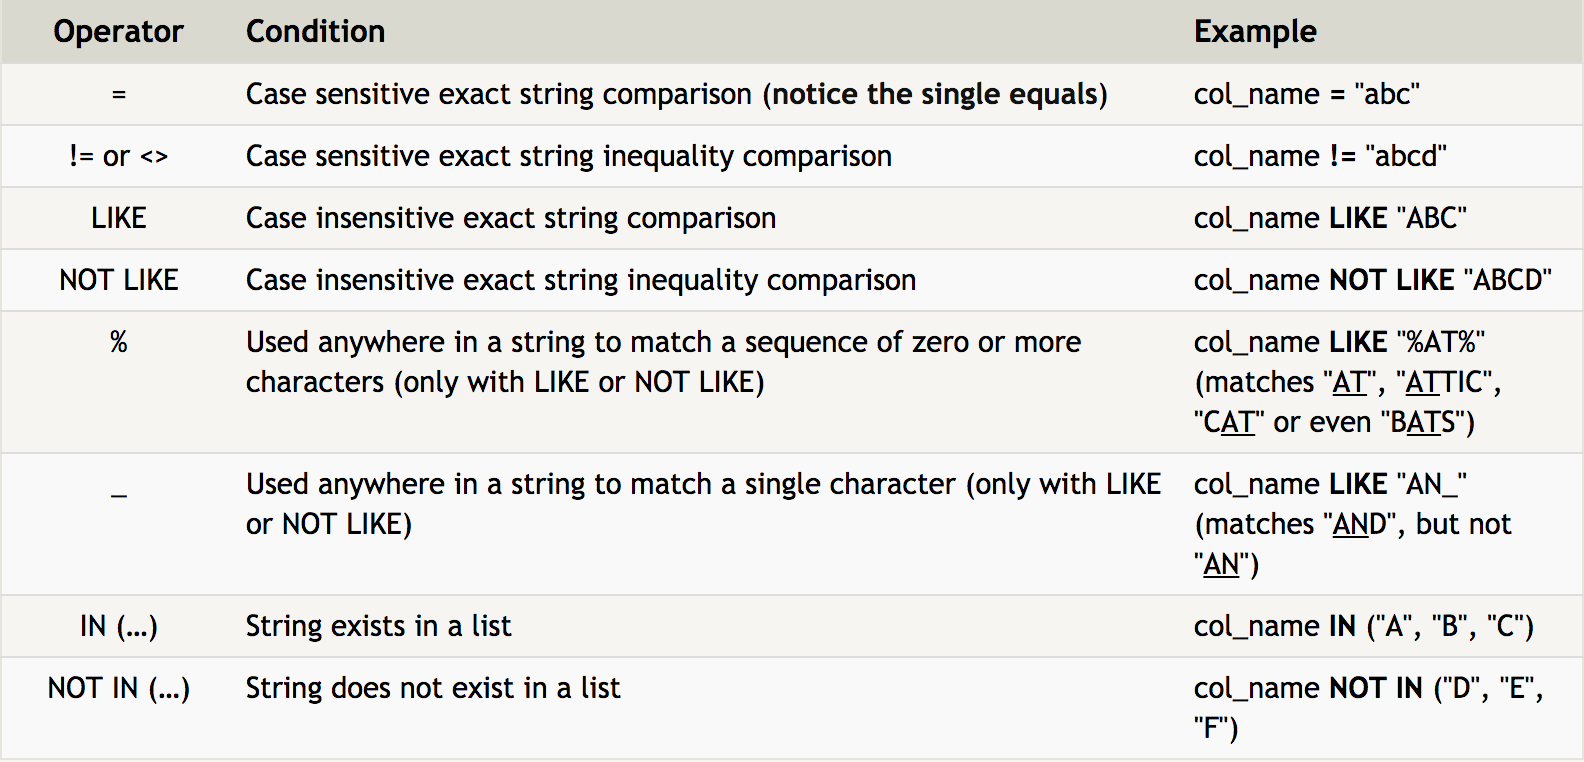
\includegraphics[width=14cm]{operators2.png}
                \end{center}
            \end{figure}

	Screenshots taken from SQLBolt! 
	


% Don't forget this line in order to increment the exercise counter
\nextexercice

%******************************************************************************%
%                                                                              %
%                             THE SQL PISCINE LOL                              %
%                                                                              %
%******************************************************************************%

\chapter{Day \exercicenumber: SLOWLY BECOMIN' POWERFUL IN SQL }
\extitle{SQL subqueries, GROUP BY, aggregate functions, HAVING}
\exfiles{04\_subquery.rb, 05\_aggregates.rb, 05a\_aggregates.rb}
\exnotes{Make sure to use docker cp to store your files on the host computer, then add it to a git repo after!}
\makeheaderfiles
 
            \begin{figure}[H]
                \begin{center}
                    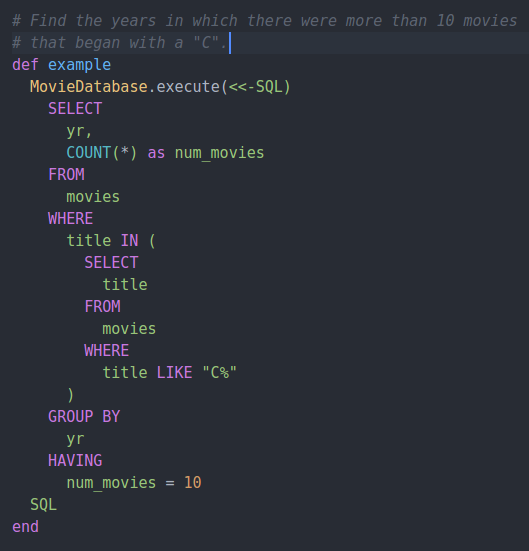
\includegraphics[width=10cm]{subquery.png}
                \end{center}
            \end{figure}

	\begin{itemize}\itemsep1pt 
		\item Subqueries are easy, aren't they? It's just a query inside of another query! 
			However, think about the type of subquery: is it correlated? A correlated 
			subquery is where the subquery is dependent on a column from the outer query, 
			meaning it runs repeatedly. 
		\item GROUP BY groups the same column results together, allowing you to use aggregate functions. 
			What happens when you use GROUP BY on more than one column? 
		\item HAVING is just like WHERE, but it happens after the GROUP BY rather than before. 
			We'll get to SQL's logical order 
			later, for now-- just know that SQL's syntactical order isn't its logical order. 
		\item Aggregate functions are helpful functions you can use on groups! What are some of the most 
			commonly used ones?
		\item If you look carefully, the text says "Find the years in which there were more than 10 movies", 
			but I only put HAVING num\_movies = 10. This error was merely a test to see your 
			level of astuteness. 
	\end{itemize}

            \begin{figure}[H]
                \begin{center}
                    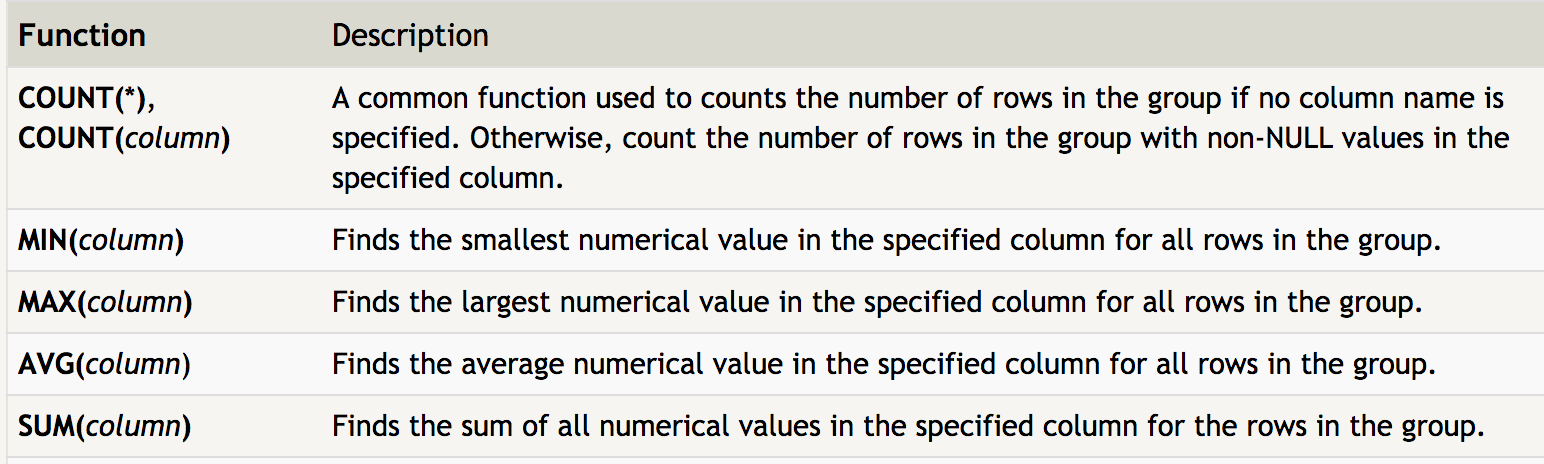
\includegraphics[width=14cm]{aggregate_functions.png}
                \end{center}
            \end{figure}

	   Another chart from SQLBolt!

% Don't forget this line in order to increment the exercise counter
\nextexercice

%******************************************************************************%
%                                                                              %
%                             THE SQL PISCINE LOL                              %
%                                                                              %
%******************************************************************************%

\chapter{Day \exercicenumber: YOUR POWER LEVEL IS RISING. }

\extitle{SQL JOINS, ORDER BY, LIMIT, join tables, primary key, foreign key, DB schema}
\exfiles{06\_joins.rb, 07\_joins.rb, 07a\_joins.rb}
\exnotes{Make sure to use docker cp to store your files on the host computer, then add it to a git repo after!}
\makeheaderfiles

            \begin{figure}[H]
                \begin{center}
                    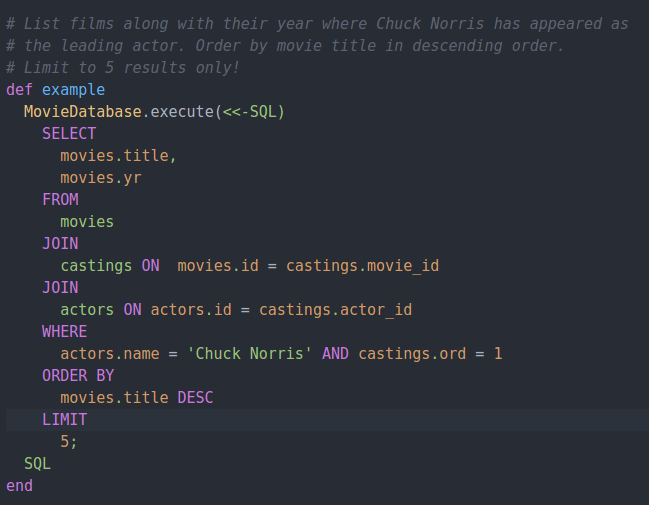
\includegraphics[width=13cm]{join.png}
                \end{center}
            \end{figure}

	\begin{itemize}\itemsep1pt 
		\item What does a JOINS do? It combines rows from two or more tables together! 
		\item ORDER BY orders your results based on some specific column, with options ASC or DESC
		\item LIMIT simply limits the amount of results you'll get back to a certain number
		\item A schema is basically just a view of the entire database 
		\item Primary keys are used to uniquely identify each row in the table. 
		\item Foreign keys are used to join two tables together!
		\item If an employees table has a boss\_id foreign key, employees will belong to boss while boss will have 
			many employees. 
		\item A join table is needed to deal with a many-to-many relationship! Think about it for a lil' bit. 
			Why is a join table needed? 
	\end{itemize}

	Rather than posting an image of what happens on a regular join, here is a link to a \href{https://blog.codinghorror.com/a-visual-explanation-of-sql-joins/}{visual representation 
	of SQL joins}.
% Don't forget this line in order to increment the exercise counter
\nextexercice

%******************************************************************************%
%                                                                              %
%                             THE SQL PISCINE LOL                              %
%                                                                              %
%******************************************************************************%

\chapter{Day \exercicenumber: AND THIS IS TO GO FURTHER BEYOND }

\extitle{SQL IS NULL/NOT NULL, OUTER JOINS, COALESCE, CASE, self joins, ternary logic}
\exfiles{08\_null.rb, 09\_self\_joins.rb, wrapper program}
\exnotes{Make sure to use docker cp to store your files on the host computer, then add it to a git repo after!}
\makeheaderfiles

            \begin{figure}[H]
                \begin{center}
                    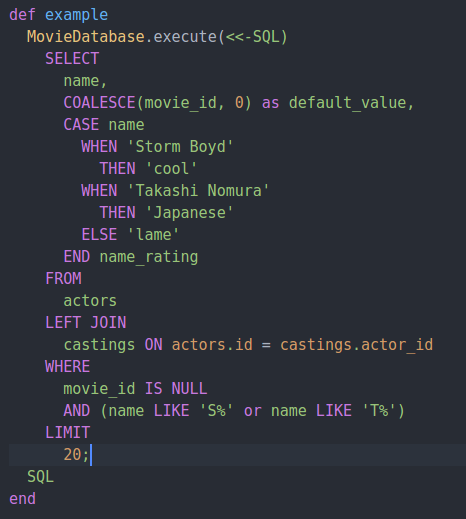
\includegraphics[width=9cm]{null.png}
                \end{center}
            \end{figure}

	\begin{itemize}\itemsep1pt 
		\item Why do you have to use IS NULL/IS NOT NULL instead of just = or != NULL? 
			Recall that NULL is unknown, so if you compare NULL = NULL, you get false 
			since they're both unknown. 
		\item Outer joins! Look above to the visual representation of SQL joins. Think about 
			why outer joins can result in NULLs. 
		\item CASE statement is self explanatory
		\item COALESCE is used to fill out NULL values with default ones!   
		\item In what cases would you use self joins and why?  
		\item What is SQL's ternary logic? -> True, false, null
	\end{itemize}

	Look at this example of a basic wrapper program! \\ 
	This is pretty poor, though. I had to use the main Object to get all the methods! 
	I'd say when you create your own DB, you should wrap up all your methods into some 
	sort of object. \\ 

	\begin{figure}[H]
		\begin{center}
			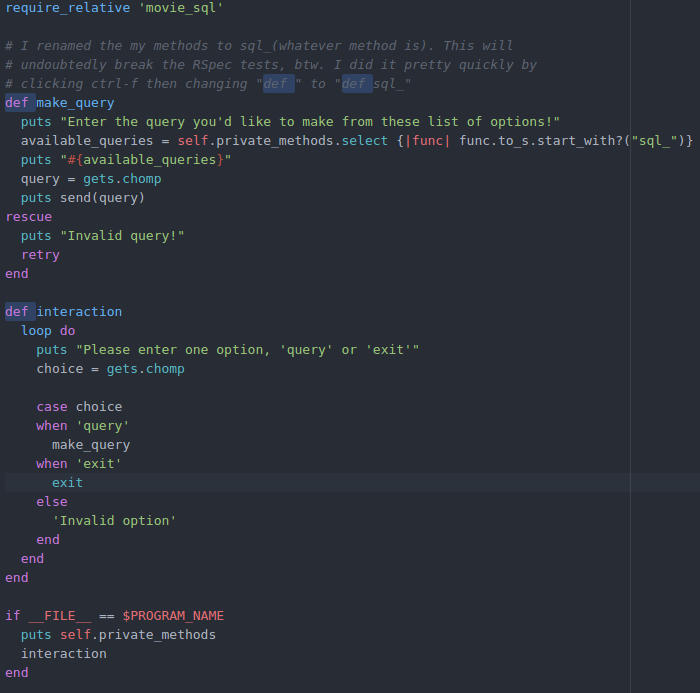
\includegraphics[width=15cm]{wrapper.png}
		\end{center}
	\end{figure}

% Don't forget this line in order to increment the exercise counter
\nextexercice


%******************************************************************************%
%                                                                              %
%                                 Bonus part                                   %
%                                                                              %
%******************************************************************************%
\chapter{Bonus part}
	Well, the first bonus is the same as the last project! It's simply to write your 
	own query questions, the solution to said questions, and a test to check if the 
	solution is correct. Write 5 of these and you'll get all the bonus points! \\ 

	If your material is good, it'll be added to the curriculum to make the 
	next gen of H2S SQL students suffer. The more work the better, right? \\ 

	Anyhow, the second bonus is much more fun. It's basically just adding extra 
	features to your wrapper program or making it look pretty. Something that would be 
	cool would be letting users interact with your database through a website or API. \\ 

	Oi oi, learn some Ruby on Rails from H2S and let's implement some good ol' MVC 
	architecture applications and websites. Or you could be lame and learn Flask instead! 

	\begin{figure}[H]
		\begin{center}
			
\includegraphics[width=12cm]{flask.png}
		\end{center}
	\end{figure}

%******************************************************************************%
%                                                                              %
%                           Turn-in and peer-evaluation                        %
%                                                                              %
%******************************************************************************%
\chapter{Turn-in and peer-evaluation}
    Turn your work in using your \texttt{GiT} repository, as
    usual. Only work present on your repository will be graded in defense. \\
	
	Remember to store all your work on a git repository-- make sure to add, commit, then push! \\ 

    Good luck and don't forget to "cd (where you stored your work) \&\& rm -rf *" once you're done.

    . \\

    . \\

    . \\ 

    . \\ 

    . \\ 

    . \\

    . \\

    . \\

    . \\
    
    . \\

    . \\
    
    . \\

    . \\

    If you've actually followed instructions and stored your work, you'll be fine.

%******************************************************************************%
\end{document}
